\documentclass{article}


% load package with some of the available options - you may not need this!
\usepackage[framed,autolinebreaks,useliterate]{mcode}

% for checklist
\usepackage{enumitem,amssymb}
\newlist{todolist}{itemize}{2}
\setlist[todolist]{label=$\square$}
\usepackage{pifont}
\newcommand{\cmark}{\ding{51}}%
\newcommand{\xmark}{\ding{55}}%
\newcommand{\done}{\rlap{$\square$}{\raisebox{2pt}{\large\hspace{1pt}\cmark}}%
\hspace{-2.5pt}}
\newcommand{\wontfix}{\rlap{$\square$}{\large\hspace{1pt}\xmark}}


% something NOT relevant to the usage of the package.
\usepackage{graphicx}
\usepackage{url,textcomp}
\setlength{\parindent}{0pt}
\setlength{\parskip}{18pt}
\title{ECTA Homework 4\\Multiobjective Optimization with the\\Non-dominated Sorting Genetic Algorithm II}
\author{\color{blue}Debaraj Barua (9030412), Md Zahiduzzaman (9030432)}
% //////////////////////////////////////////////////

\begin{document}

\maketitle


\newpage

\section{Assignment Description}
	\begin{enumerate}
		\item Implement the NSGA-II algorithm and apply it to a toy problem
			\begin{itemize}
			\item Bit string with length 20
			\item Maximize the number of leading zeros (zeros in a row at the front)
			\item Maximize the number of trailing ones (ones in a row at the back)
		\end{itemize}
		\item Show that your algorithm works by plotting the population at various stage of the algorithm
	\end{enumerate}

\section{Submission Instructions}
Follow along with the instructions in this PDF, filling in your own code, data, and observations as noted. Your own data should be inserted into the latex code of the PDF and recompiled. All code must be done in MATLAB.

To be perfectly clear we expect two submissions to LEA:
\begin{enumerate}
	\item 1 PDF (report) -- a modified version of your submission PDF, with your own code snippets, figures, and responses inserted
	\item 1 ZIP (code and data)   -- a .zip file containing all code use to run experiments (.m files) \textit{and} resulting data as a .mat file
	\item 1 GIF (algorithm progress) -- use the file on the MATLAB file exchange: \url{https://www.mathworks.com/matlabcentral/fileexchange/63239-gif}
\end{enumerate}


\newpage
\section{The Assignment}

\subsection{NSGA-II (75pts)}
\begin{itemize}
	\item (50pts) Implement NSGA-II to find all non-dominated solutions to the trailing ones, leading zeros problem. 
	\begin{itemize}
		\item Bitstring with length 20
		\item Population size of 100
		\item Generations 100
		\item Hints:
		\begin{itemize}
			\item Crossover and mutation can be performed just as in other bit string problems, e.g. one-max
			\item The \mcode{sortrows} function can be used to sort matrices, you can use this first before implementing NSGAs sorting
		\end{itemize}
	\end{itemize}
	\item (20pts) Visualize the progress of your algorithm over a single 100 generation run with an animated gif (1 frame every generation).
	\begin{itemize}
		\item Use the code here: \url{https://www.mathworks.com/matlabcentral/fileexchange/63239-gif} to create gif
		\begin{itemize}
			\item Set the timing so that the gif completes in a reasonable amount of time (between 10 and 20 seconds)
		\end{itemize}
		\item Fronts can be visualized with the code snippets attached\\ (\mcode{displayFronts.m})
	\end{itemize}
	{\color{blue} The visualization is shown in plot.gif and submitted with the assignment}
	\item (5pts) At each iteration mark the individuals which carry on to the next population, and which do not (you will have to code this yourself).\\
	{\color{blue} Individuals carried to the next population is marked as green circle and others are marked as red circle. The individuals at the first front are marked as filled circle}
\end{itemize}

\newpage
\subsection{Short Answer (25pts)}
\begin{itemize}
	\item (10pts) Compare the sort used by NSGA-II with a variety of population sizes. How long does 100 generations take with each approach when using a population size of:
	\begin{enumerate}
		\item 10: {\color{blue}25.6265 seconds, does not find any of the pareto optimal solution.}
		\item 100: {\color{blue}50.1688 seconds, finds all 21 pareto optimal solutions.}
		\item 1000: {\color{blue} 1828.7204 seconds, The population size is too high because with genome of length 20 there can be only 210 unique solutions ($\frac{N \times (N+1)}{2}$) and population size of larger then this is not helpful.}
	\end{enumerate}
	
	
	\item (5pts) Plot the end result of a single run with [100 pop and 100 gen] and [10 pop and 1000 gen]. Describe the difference between the end results. Which is preferable? \\

	\begin{figure}[h]
		\centering
		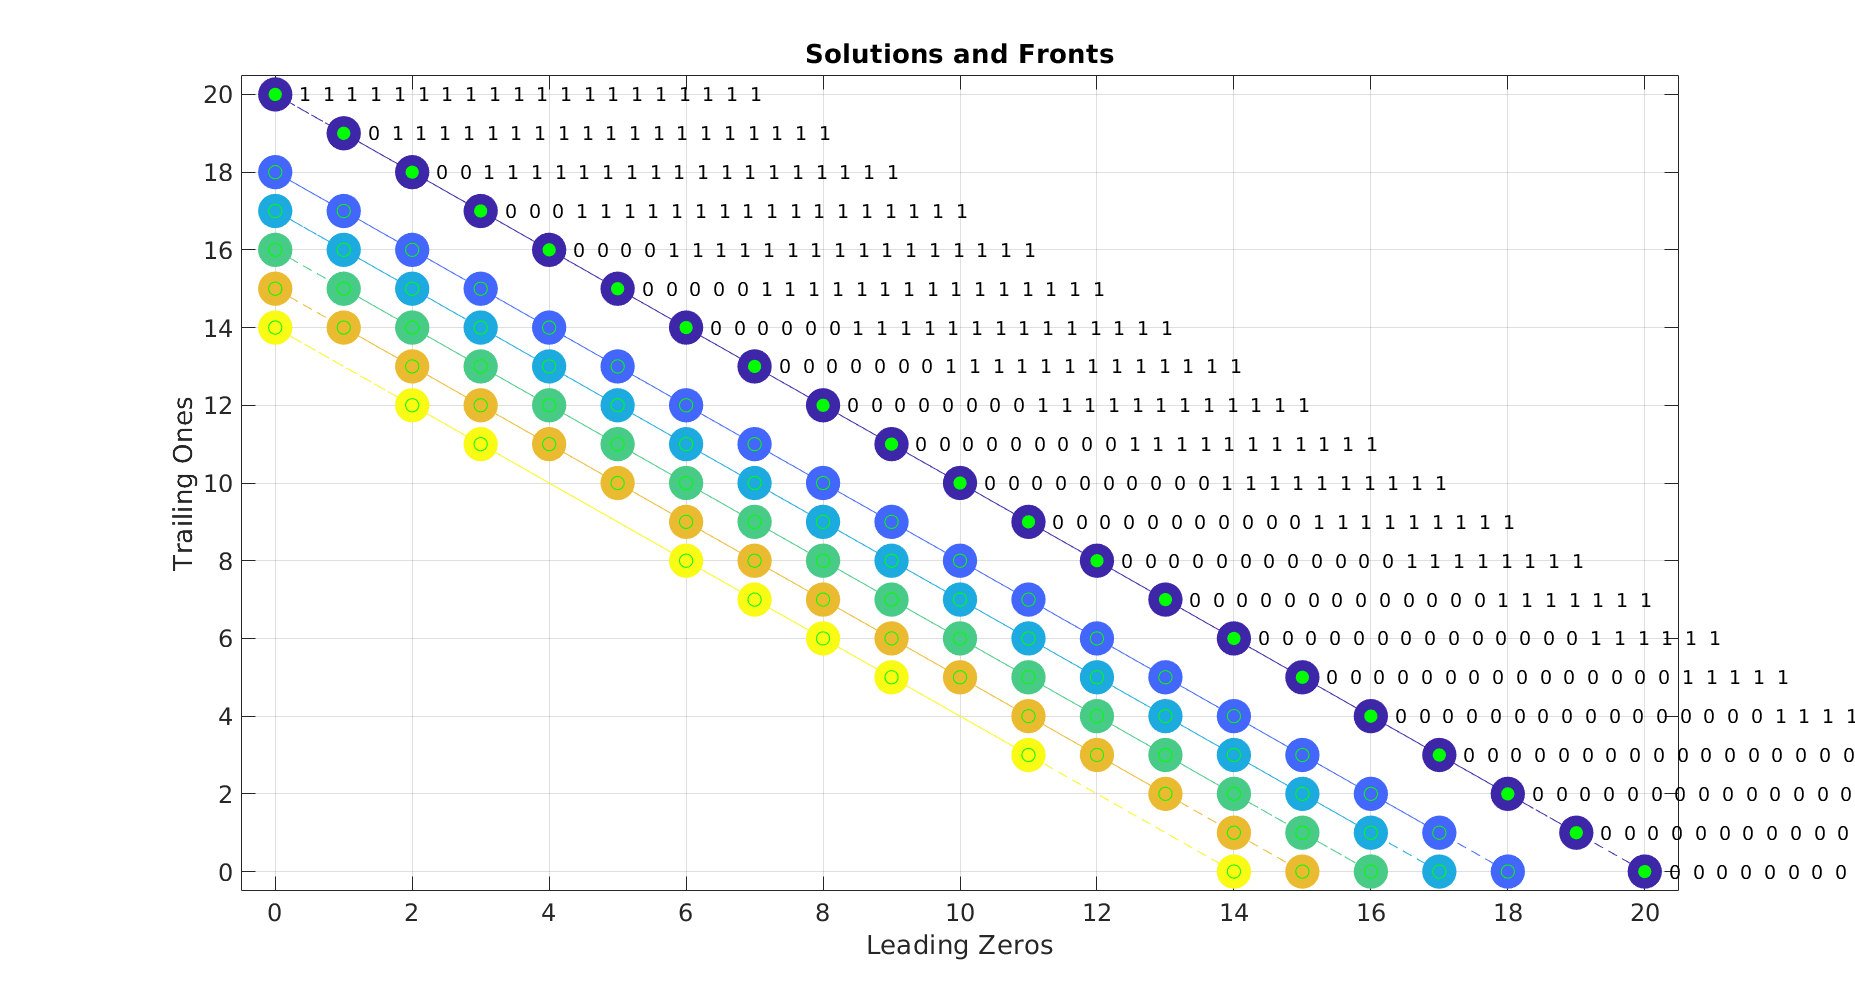
\includegraphics[width=0.7\linewidth]{img/p_100_g_100}
		\caption{pop 100, gen 100, takes 53.5034 seconds}
		\label{fig:p_100_g_100}
	\end{figure}
	
	\begin{figure}[h]
		\centering
		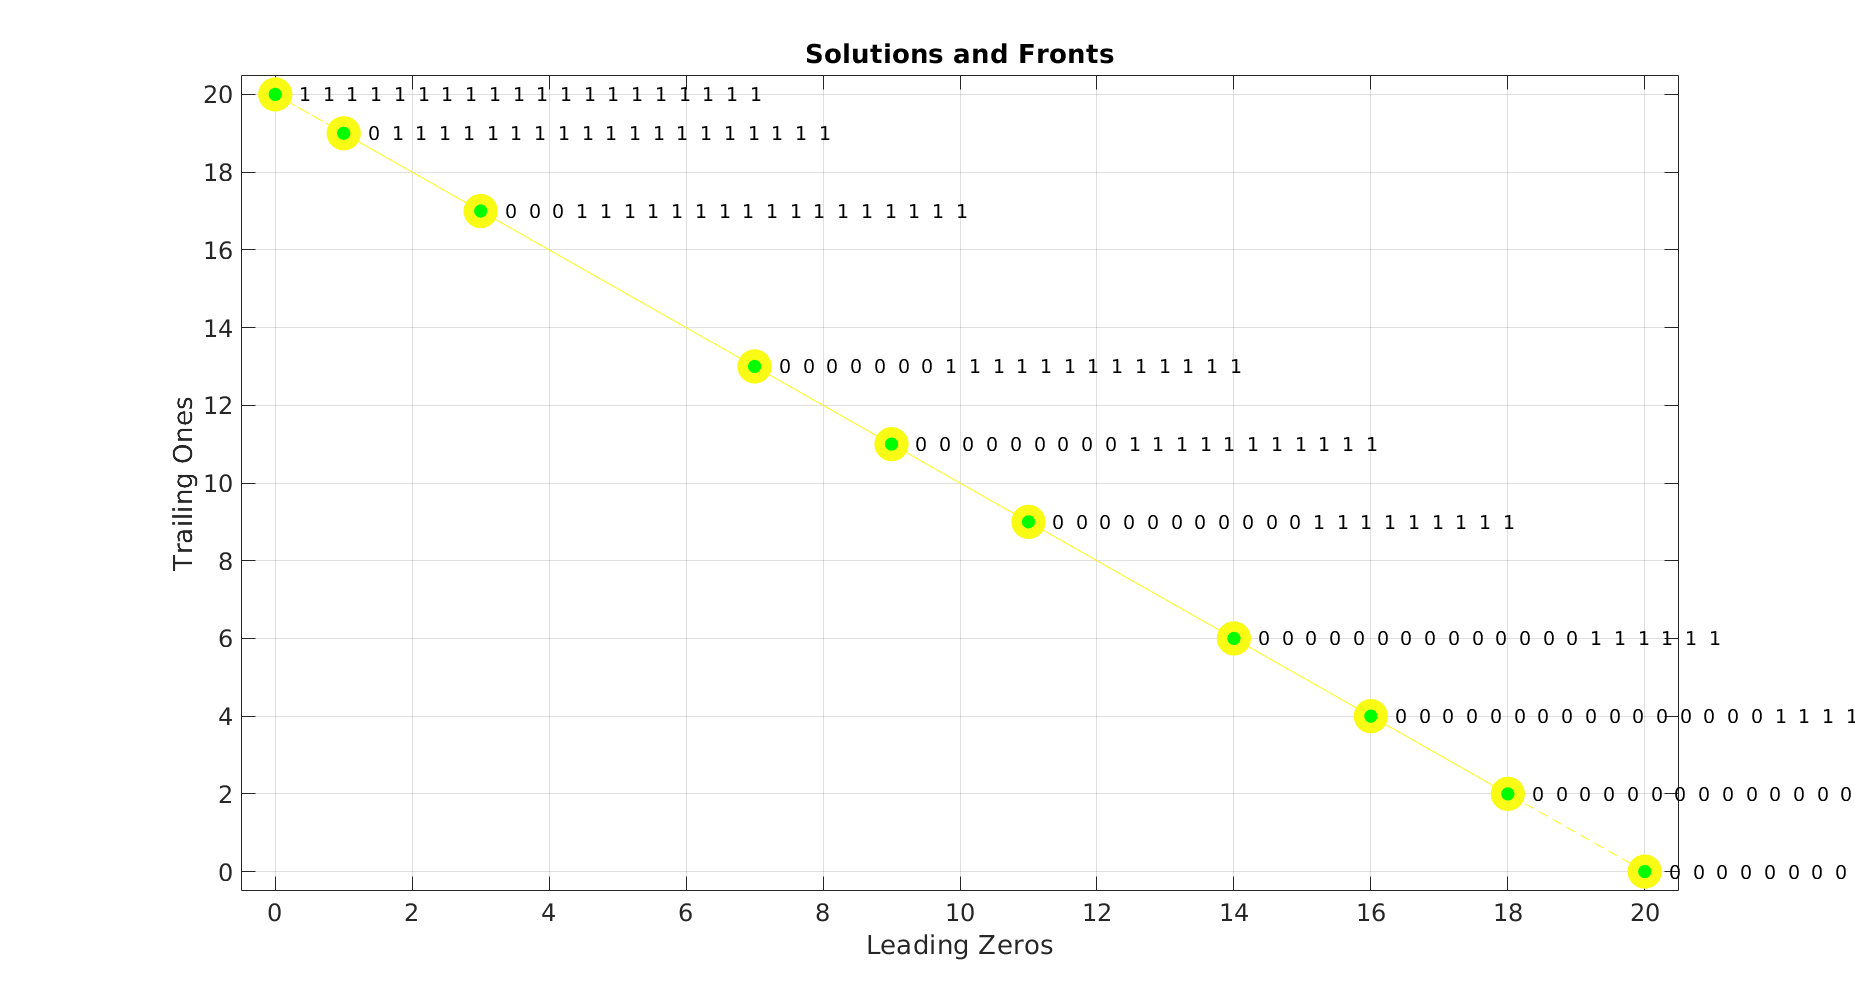
\includegraphics[width=0.7\linewidth]{img/p_10_g_1000}
		\caption{pop 10, gen 1000, takes 233.6489 seconds}
		\label{fig:p_10_g_1000}
	\end{figure}
	

	
	{\color{blue}The end result shows that due to the small population size in case of population size 10, it does not find all 21 pareto optimal solutions and it takes longer to run. So, pop 100 and gen 100 is better.}
	
	\item (5pts) Imagine you were to replace the objective of ``leading zeros'' with ``largest binary number''. Predict the result, and give your reasoning.\\
	{\color{blue}In this case there will be only one pareto optimal solution which is a bit string of 1's of length 20. In this case both the objectives will have value 20 and no other individual can dominate this individual.}
	\item (5pts) Imagine you were to add a third objective: ``non-consecutive ones and zeros'' (ones not touching ones and zeros not touching zeros, e.g. 0101 and 1010 are the most optimal 4 bit solutions). How would you adjust the hyperparameters to get a satisfactory result?\\
	{\color{red}Will answer after extra credit task}
	\item (5pts) In many GAs and ESs populations must be ranked, but no special methods are used. Why is a faster sort in MOO so important?\\
	{\color{blue}A faster sort is important because of the the number of comparison performed and less comparison requires less time and vice versa. The approach we followed requires $\mathcal{O}(M N^2)$ whereas a naive implementation is also possible which is easier to implement but requires $\mathcal{O}(M N^3)$ comparison operations. Here $M$ is number of objectives and $N$ is the population size. It makes a huge difference for large population size.}
\end{itemize}

\newpage
\subsection{** Extra Credit ** (+ 10pts in examination)}
Implement the third objective ``non-consecutive ones and zeros''
\begin{enumerate}
	\item How many non-dominated solutions are possible? (Hint: start with a smaller length and test)
	\item What changes did you make to the algorithm and hyperparameters to get a good result?
	\item List the solutions in your 1st front. Are they all Pareto optimal? How complete is your front (in percentage, based on $\#1$)
	\item Plot the end result in 3D. (Use \mcode{plot3} or \mcode{scatter3})
\end{enumerate}


\end{document}














